\documentclass[a4j, 11pt]{jarticle}
\usepackage{graphicx}
\usepackage{titling}
\usepackage{amsmath}
\usepackage{float}
\usepackage{listings}
\usepackage{booktabs}
\usepackage{siunitx}
\usepackage{makeidx}

\renewcommand{\lstlistingname}{コード}
\graphicspath{{./assets/}}
\title{様々なソートアルゴリズム}
\author{クリスティアン ハルジュノ\thanks{釧路工業高等専門学校情報工学科5年情報21番}}
\date{\today}
\begin{document}
\begin{titlepage}
  \centering
  \vspace*{3cm}

  {\fontsize{25pt}{36pt}\selectfont\bfseries ソートプログラム} \\[1cm]  % Main title
  {\Large 釧路工業高等専門学校情報工学科5年・情報工学実験II} \\[1cm]
  {\large 氏名:クリスティアン・ハルジュノ} \\[1cm]
  {\large 出席番号:21} \\[1cm]
  {\large 学籍番号:234071} \\[5cm]


  {\Large 提出日:2025年6月17日} \\

  \vfill

\end{titlepage}
\tableofcontents
\newpage
\setcounter{page}{1}
\section{初めに}
データに最適なソートアルゴリズムを選択するのは容易ではない. Big-O記法を用いて理論的にアルゴリズムを比較することは可能であるが, 現実のソートアルゴリズムはそれ以上の要素を含んでいる\cite{energo2023bigoh}. \\

理論的に効率的なアルゴリズムの中には, 実装前に徹底的に調査する必要がある弱点を持つものもある. 一部のアルゴリズムは, データがアルゴリズムを最適に実行できる特定の状態にある場合にのみ効率的である. \\

現代のコンピュータは, 大容量メモリ, 高速CPU, 効率的なストレージなど, 十分なハードウェアスペックを備えているが, 一部のアルゴリズムは高速実行のためにリソースを犠牲にしている. データサイズが小さい場合は, これは問題にならないかもしれない. しかし, ビッグデータ企業のようにデータを大規模化すると, リソースは適切に対処する必要がある非常に重要な問題になる. そのため, アルゴリズムを理論的に比較するだけでなく, 対象データセットに対してこれらのアルゴリズムをテストし, 結果を分析することが重要である. \\

本レポートでは, 実装が最もシンプルなものからより複雑なものまで, 最も普及している6つのソートアルゴリズムを検証し, 7つの固定データセットと比較する. 各データセットには, 1から50000までの整数が10万行含まれている. 各データセットは, 完全にランダム, 反転, ソート済みなど, さまざまな段階にある. これらの比較により, 選択した6つのソートアルゴリズムの長所, 短所, および動作を検証できる. \\
\section{背景}
このセクションでは, この実験で使用した6つのソートアルゴリズムを紹介し, それぞれがどのように機能するかを説明する.
\subsection{ソートアルゴリズムを紹介}
\begin{description}
  \item[バブルソート] バブルソートは最もよく知られているソートアルゴリズムの一つである. 実装が非常に簡単であり, 少量のデータに対してはメモリ使用量が少なく, 処理も比較的高速である. この方法にはデータを最初から最後まで調べながら, 現在の数値と次の数値を比較することで機能する. 現在の数値が次の数値よりも大きい場合は, 位置を入れ替える. このプロセスは, データが完全にソートされるまで何度も繰り返される\cite{friend1956sort}.\\
  \item[シェーカーソート] シェーカーソートまたはカクテルソートはバブルソートと似てるであるが, シェーカーソートでは左から右に移動だけでなく逆向きにもう通過する\cite{shaker1961cocktail}. \\
  \item[挿入ソート] 挿入ソートは, 要素を適切な位置に直接挿入することで並べ替えを行うアルゴリズムである. 現在処理している要素を, それより前の要素と右から左に1つずつ比較し, 比較対象が現在の要素より大きければ, 右にずらす. 適切な位置が見つかったところで, 現在の要素を挿入する\cite{knuth1998insertion}. \\
  \item[バケットソート] バケットソートは他方法より速度が最高と言える. しかし, ソートの高速にはメモり使用量の増加が伴う. バケットソートでは, データを複数のバケットに分割しする. 各バケットは, バブルソートや挿入ソートなどの手法を用いてソートされる. すべての要素を指定されたバケットに挿入した後, すべてのバケットを連結してソート済みの配列を作成する. この手法は, 大規模なデータに対して単純なソートアルゴリズムを実行する必要がないため, 高速である. 前述のように, バブルソートなどの一般的なソート手法は, 大規模なデータベースではパフォーマンスが低下する. しかし, 少量のデータであれば問題ない. データを独自のバケットに分割することで, 1回の操作で処理しなければならないデータ量が大幅に削減され, アルゴリズムの負荷が軽減される\cite{corwin2004bucket}. \\
  \item[クイックソート] クイックソートは分割統治ソートと言われている. このソート方法ではある配列から枢軸を選び, 全要素をその枢軸に比較する. 枢軸より小さいとその要素を枢軸の左がわにづらす. 枢軸より大きいと, その要素を枢軸の右側にづらす. 枢軸を分岐点とし, 配列を左配列と右配列に分割する. この処理を各文割された配列に対応し, 繰り返して行う. 最小配列に着くと, 各配列をまた分岐点枢軸の左と右側に繋ぎる\cite{hoare1961quicksort}. \\
  \item[カウントソート] バケットソートと似たように, このソート方法でもバケットのような配列を作成する. まず, データ配列内の最大値を探索し, その値をもとにカウント配列(頻度を格納するための配列)を作成する. 次に, 元のデータ配列を1つずつ走査し, それぞれの値に対応するインデックスのカウント配列の値をインクリメントすることで, 各値の出現回数を記録する. その後, カウント配列を累積和に変換し, それをもとに元のデータを安定的に新しい配列へと並べ替えていく. このソートは整数値に限定されるが, 非高速でソートできる\cite{seward1954counting}. \\
\end{description}

\subsection{理論的な比較}
表\ref{tab:sort-comparison}, セクション2.1で前述した各ソート手法の基本的な特性または動作を示している. 各アルゴリズムの特性は, 最良の計算複雑度, 平均的な計算量, 最悪の計算量に分類される. 最良の計算量は, 特定の入力状態においてデータをソートするために必要な最小の演算量を表す. 平均的な計算量は, 考えられるすべての入力を考慮し, データをソートするために必要な予想される演算量を表す. 最悪の計算量は, 特定の入力状態においてデータ処理に必要な最大の時間を表する.
\begin{table}[htbp]
  \centering
  \caption{各ソートアルゴリズムの計算量と特徴の比較}\label{tab:sort-comparison}
  \resizebox{\linewidth}{!}{%
    \begin{tabular}{|l|c|c|c|c|c|c|}
      \hline
      \textbf{アルゴリズム} & \textbf{最良計算量} & \textbf{平均計算量} & \textbf{最悪計算量} & \textbf{空間計算量} & \textbf{インプレース} \\
      \hline
      バブルソート\cite{gfg:bubblesort2024}     & $O(n)$          & $O(n^2)$         & $O(n^2)$         & $O(1)$            & はい \\
      シェーカーソート\cite{gfg:cocktailsort2024}   & $O(n)$          & $O(n^2)$         & $O(n^2)$         & $O(1)$           & はい \\
      挿入ソート\cite{gfg:insertionsort2024}         & $O(n)$          & $O(n^2)$         & $O(n^2)$         & $O(1)$           & はい \\
      バケットソート\cite{gfg:bucketsort2024}     & $O(n + k)$      & $O(n + k)$       & $O(n^2)^\dagger$ & $O(n + k)$       & いいえ \\
      クイックソート\cite{gfg:quicksort2025}     & $O(n \log n)$   & $O(n \log n)$    & $O(n^2)$         & $O(\log n)^*$   & はい \\
      カウントソート\cite{gfg:countingsort2024}     & $O(n + k)$      & $O(n + k)$       & $O(n + k)$       & $O(k)$           & いいえ \\
      \hline
    \end{tabular}
  }
\end{table}

計算量を指定するために, Big O表記法を使用する. Big O表記法は, 処理する必要があるデータの量に基づいてソート アルゴリズムのパフォーマンスを評価する最も基本的な方法の1つである\cite{energo2023bigoh}. 表\ref{tab:sort-comparison}に示されているように, バブルソート, シェイカーソート, 挿入ソートの平均計算量は$O(n^2)$である. Big O表記法では, $n$はデータ自体の長さに対応する. データのソートに必要な操作数に対して$n$をプロットすると, 計算量が$O(n^2)$の図\ref{bigograph}に示すように, ソートするデータの数がわずかに変化するだけでも操作数が大幅に増加し, 大量のデータのソート効率が低下する可能性がある. しかし, 計算量が$O(n \log n)$のクイックソートを\ref{bigograph}と比較すると, データ量を大幅に増やした場合でも, 特定のデータをソートするために必要な操作の量は, 複雑度が$O(n^2)$のアルゴリズムに比べてはるかに少なくなる.\\

上記のアルゴリズムの最良計算量について, バブルソート, シェイカーソート, 挿入ソートはいずれも, 与えられた入力データが既にソート済みであることを前提としている. この場合, アルゴリズムはデータを1回だけ処理すればよいため, 計算量は$O(n^2)$から$O(n)$に減少する. バケットソート最良計算量では, すべての要素が各バケットに均等に分散されていると想定される. クイックソートの最良計算量では, ピボットの選択によって値が左右に均等に分散されると想定される. 最後に, カウントソートの最良計算量では, 入力データの整数の範囲が狭いと想定される. \\

最後に, 外部配列を用いてデータの内容をソートするバケットソートとカウントソートの場合, 平均的な計算量は$O(n + k)$で測定される. ここで, $k$は外部配列の処理に必要な演算量を表す. $k$を調整することで, 特定のデータのソートに必要な演算量を大幅に削減可能性がある.\\

\begin{figure}[H]
  \centering
  \includegraphics[width=0.8\linewidth]{bigo.eps}
  \caption{様々な計算量を比較}\label{bigograph}
\end{figure}

表\ref{tab:sort-comparison}に基づくと, 空間計算量とインプレースは, ソートが元のデータ配列自体の外で行われることを指す. バブルソート, シェイカーソート, 挿入ソートの空間計算量が$O(1)$ので, 与えられたデータをソートするために必要な空間の量は最初から変わらない. つまり, これらのアルゴリズムは非常に空間効率が高く, 元のデータとは別に新しいメモリを割り当てる必要がない. バケットソートとカウントソートのアルゴリズムの空間計算量は$O(n + k)$と$O(k)$であり, この場合, $k$はデータをソートするために作成される新しい空間の量を指す. これらのアルゴリズムは新しい空間を割り当てる必要があり, アルゴリズムの設定方法によっては大量のメモリを消費する可能性がある. クイックソートは特に注目すべき点である. クイックソートの空間計算量は$O(\log n)$であるが, すべての操作はデータ配列内で行われ, 新しいメモリを割り当てる必要はない. そのため, クイックソートはインプレースソートアルゴリズムと呼ばれる. クイックソートはソートが進むにつれて, 処理が必要なデータの長さが縮小し続けるためである.\\

\section{実験セットアップ}
\subsection{ハードウェアと環境}
ハードウェアとしてはAppleシリコンのプロセッサに基づいて実験を行う. 
\begin{description}
  \item[機種名] Apple Macbook Pro (M3, 2023年モデル)
  \item[プロセッサ] Apple M3チップ(8コア:高性能コア4+高効率コア4)
  \item[GPU] 10コア統合型GPU
  \item[メモリ] 16GBユニファイドメモリ
  \item[ストレージ] 1TB SSD
  \item[OS] macOS Sequoia 15.5
  \item[アーキテクチャ] ARM64(Appleシリコン) 
\end{description}
また, 作成した実験プログラムはC言語で書き, GCCコンパイラでコンパイルされる. 
\begin{verbatim}
  Apple clang version 17.0.0 (clang-1700.0.13.5)
  Target: arm64-apple-darwin24.5.0
  Thread model: posix
\end{verbatim}
コンパイルを効率化するため, GCCコンパイラをMakeと同時に利用する. 
\begin{verbatim}
  GNU Make 3.81
  Copyright (C) 2006  Free Software Foundation, Inc.
  This is free software; see the source for copying conditions.
  There is NO warranty; not even for MERCHANTABILITY or 
  FITNESS FOR A PARTICULAR PURPOSE.
  This program built for i386-apple-darwin11.3.0
\end{verbatim}
\subsection{実験に使用するデータセット}
各ソート アルゴリズムの制限と動作を適切にテストするために, 1 から 50000 までの範囲の 100000 個の整数を含む 7 つのデータセットを用意した. 各データセットの構造は, 適用されたソート アルゴリズムの動作を引き出すためにさまざまな方法で配置されている. 
\begin{table}[htbp]
  \centering
  \caption{各データファイルの内容}
  \begin{tabular}{|c|c|c|}
    \hline
    ファイル名 & データ数 & データの種類 \\
    \hline
    data1.dat & 100,000 & ランダムデータ \\
    data2.dat & 100,000 & ランダムデータ \\
    data3.dat & 100,000 & ランダムデータ \\
    data4.dat & 100,000 & 昇順データ \\
    data5.dat & 100,000 & 降順データ \\
    data6.dat & 100,000 & バイトニックデータ \\
    data7.dat & 100,000 & ジグザグデータ \\
    \hline
  \end{tabular}\label{tab:dataset-summary}
\end{table}
表\ref{tab:dataset-summary}を見ると, データセット1から3にはすべて10万個の整数が含まれており, それらはランダムに並べられていることがわかる. データセット4には, 適用されたアルゴリズムの最良のシナリオをシミュレートするために既にソートされたデータが含まれている. データセット5は, ソートアルゴリズムの最悪のシナリオをシミュレートするために, 逆順にソートされている. \\

データセット6はバイトニックシーケンスで配置されている. 数式\ref{bitonicsequence}により, バイトニックシーケンスとは, データセットの先頭から緩やかに上昇し, 中央でピークに達し, その後, データセットの末尾に近づくにつれて緩やかに下降するデータと説明できる. \\
\begin{equation}\label{bitonicsequence}
a_1 < a_2 < \cdots < a_k > a_{k+1} > \cdots > a_n
\quad (1 \leq k < n)
\end{equation}

データせっと6の先頭付近と中間付近と末尾付近からサンプル要素をランダム的に取って, 表\ref{tab:data6-sample}のようになる. 
\begin{table}[H]
  \centering
  \caption{バイトニックデータ(data6.dat)のサンプル値}
  \begin{tabular}{|c|c|}
    \hline
    位置 & サンプル値(例) \\
    \hline
    先頭付近 & 17131, 41279, 23264, 44242, 2505, 6637, 5374,\\
    中間付近(最大付近) & 43248, 43247, 43247, 43246, 43244 \\
    末尾付近 & 12, 12, 10, 10, 9, 9, 9, 9, 8, 8, 7, 5, 2 \\
    \hline
  \end{tabular}\label{tab:data6-sample}
\end{table}

データセット7はジグザグ配列になっている. 数式\ref{tab:data7-sample}ジグザグ配列とは, データ全体を通して小さな数値と大きな数値が交互に現れるデータのことである. この場合, データセットはランダム化され, 「小さい」部分と「大きい」部分が交互に現れる. データセットは, これらの大きな部分と小さな部分が, 長さを変えながら交互に現れる. \\
\begin{equation}\label{zigzagsequence}
  a_1 < a_2 > a_3 < a_4 > a_5 < \cdots
\end{equation}
データせっと7の先頭付近と中間付近と末尾付近からサンプル要素をランダム的に取って, 表\ref{tab:data6-sample}のようになる. 
\begin{table}[H]
  \centering
  \caption{ザクザクデータ(data7.dat)のサンプル値}
  \begin{tabular}{|c|c|}
    \hline
    位置 & サンプル値(例) \\
    \hline
    先頭付近 & 2, 2, 2, 4, 7, 7, 7, 8, 13, 15 \\
    中間付近 & 20778, 42992, 29869, 31747, 22945, 40054, 38945, 47166 \\
    末尾付近 & 11990, 7746, 38998, 35057, 41719, 22808, 23284, 2525\\
    \hline
  \end{tabular}\label{tab:data7-sample}
\end{table}
\subsection{測定について}
ソートアルゴリズムの実行時間を正確に測定するために, C言語の$time.c$ライブラリを利用する. $time.h$ライブラリには, プログラム実行後に経過したCPUティック数を測定する$clock()$関数が用意されている\cite{ibm:clock2024}. 図\ref{fig:clockcode}により, $clock()$関数を使用することで, ソート関数の実行前から完了後までのティック数を測定する. 得られたティック数を, CPUが1ティックを実行するのにかかる時間で割る. この値を計算すると, ソート関数の合計実行時間が算出される. 
\begin{figure}[htbp]
  \centering
  \caption{プログラムの測定分の例}\label{fig:clockcode}
  \begin{lstlisting}[basicstyle=\ttfamily\small]
    start_time = clock();
    shakerSort(fileLength, clonedArray);
    end_time = clock();
    elapsed_time = (double)(end_time - start_time)
                    /CLOCKS_PER_SEC;
  \end{lstlisting}
\end{figure}
\newpage
\subsection{各アルゴリズムの説明}
\subsubsection{バブルソート}
\begin{enumerate}
  \item リストの最初の位置から始める. 
  \item 現在の数値と次の数値を比較する. 
  \item 現在の数値が次の数値より大きければ, 入れ替える. 
  \item 次の位置に進み, リストの末尾までステップ2〜3を繰り返す. 
  \begin{figure}[H]
    \centering
    \includegraphics[width=0.8\linewidth]{bubble1.eps}
    \caption{先頭から末尾まで数値を比較して, 交換する. }
  \end{figure}
  \item 1回の通過が終わったら, 最初の位置に戻って再び通過を行う. 
  \begin{figure}[H]
    \centering
    \includegraphics[width=0.8\linewidth]{bubble2.eps}
    \caption{通過後最初の位置に戻って, 再び通過}
  \end{figure}
  \item 通過中に1回も入れ替えがなければ, ソートは完了. 
  \item 入れ替えがあった場合, ステップ1〜6を繰り返す. 
  \begin{figure}[H]
    \centering
    \includegraphics[width=0.8\linewidth]{bubble3.eps}
    \caption{通過後に入れ替えされた要素がないと終了}
  \end{figure}
\end{enumerate}
\subsubsection{シェーカーソート}
\begin{enumerate}
  \item 配列の先頭から走査を開始する. 
  \item 現在の要素と次の要素を比較し, 現在の要素の方が大きければ交換する. 
  \item 配列の末尾まで進み, 走査中に交換が一度も行われなければソートを終了する. 
  \item 次に逆方向(末尾から先頭)に走査する. 
  \item 現在の要素と前の要素を比較し, 現在の要素の方が小さければ交換する. 
  \item 先頭まで進み, 走査中に交換が一度も行われなければソートを終了する. 
  \item 上記の操作を, 交換が行われる限り繰り返す. 各往復ごとに走査範囲を狭めることができる. 
  \begin{figure}[H]
    \centering
    \includegraphics[width=0.8\linewidth]{shaker.eps}
    \caption{シェーカーソートの進み方}
  \end{figure}
\end{enumerate}
\newpage
\subsubsection{挿入ソート}
\begin{enumerate}
  \item 最初の要素をソート済み部分とみなす. 
  \item 次の要素を取り出して, ソート済み部分の各要素と比較する. 
  \item ソート済み部分の中で, 自分より大きい要素を右にずらす. 適切な位置に挿入する. 
  \item 適切位置がないとそのままで次の位置に進む
  \begin{figure}[H]
    \centering
    \includegraphics[width=\linewidth]{insertion1.eps}
    \caption{第二位置からスタート. ソート済み要素より大きい数値を左にずらす.}
  \end{figure}
  \item リストの末尾までステップ2〜4を繰り返す. 
  \item ソートされていない要素がないと終了
  \begin{figure}[H]
    \centering
    \includegraphics[width=\linewidth]{insertion2.eps}
    \caption{ソート対象値がないとソート終了}
  \end{figure}
\end{enumerate}
\subsubsection{バケットソート}
作成するバケット数の選択は, 再現性を確保し, パフォーマンス評価の一貫性を維持するために重要であるため, 入力特性に基づいて動的に決定するのではなく, すべてのテスト実行でバケット数を固定した. 本レポートの結果の大部分では, バケット数を100としている. また, バケット数がメモリ使用量とソート速度に与える影響についても考察する. 更に, 各バケットをソートする必要があるため, 挿入ソートを利用する.\cite{gfg:bucketsort2024}\\
\begin{enumerate}
  \begin{figure}[H]
    \centering
    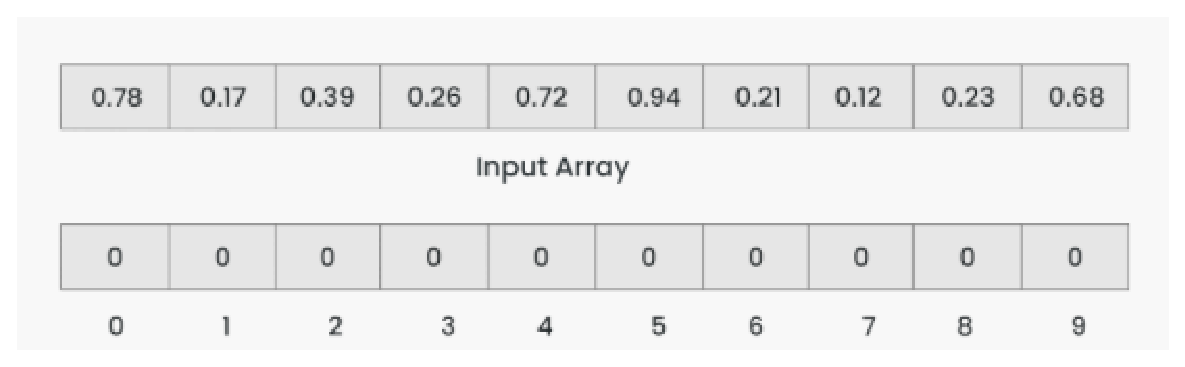
\includegraphics[width=\linewidth]{bucket1.eps}
    \caption{ソート対象データ}
  \end{figure}
  \item 最初に, ソート対象の整数の範囲(例:0〜2.5)を確認し, その範囲に応じてバケットの数を決める(例:3の範囲ごとにバケットを作成するなど). 
  \begin{figure}[H]
    \centering
    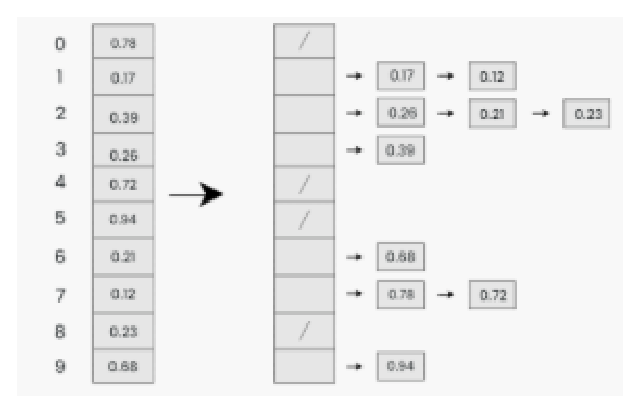
\includegraphics[width=0.8\linewidth]{bucket2.eps}
    \caption{作成したバケット}
  \end{figure}
  \item 各要素をその値に基づいて対応するバケットに振り分ける. 
  \begin{figure}[H]
    \centering
    \includegraphics[width=0.8\linewidth]{bucket3.eps}
    \caption{適当に作成されたバケットに要素を入れる. }
  \end{figure}
  \newpage
  \item 各バケット内の要素をソートする(挿入ソートやバブルソートなど, 単純なソートでOK). 
  \begin{figure}[H]
    \centering
    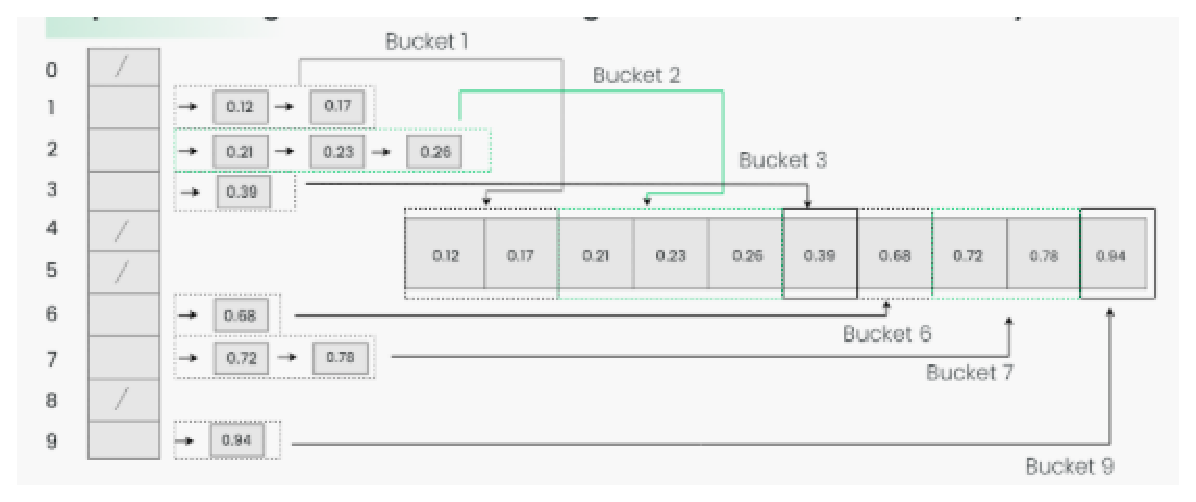
\includegraphics[width=0.8\linewidth]{bucket4.eps}
    \caption{各バケットの内容をソートし, 連続}
  \end{figure}
  \item すべてのバケットを順番に結合して, 最終的なソート済み配列を作る. 
  \begin{figure}[H]
    \centering
    \includegraphics[width=0.8\linewidth]{bucket5.eps}
    \caption{ソートずみの配列}
  \end{figure}
\end{enumerate}
\subsubsection{クイックソート}
クイックソートを利用する場合, ピボットポイントの選択はアルゴリズムのパフォーマンスに重要である. 最適なピボットポイントは, 小さい(左)配列と大きい(右)配列を均等に分割できるものである. 常に最大のピボット値または最小のピボット値を選択すると, すべてのデータ値をピボットポイントの左側または右側に移動する必要があるため, ソートアルゴリズムの効率が大幅に低下する. その結果, 計算量は$O(n \log n)$から$O(n^2)$に変化してしまう\cite{gfg:quicksort2025}. この実験では, データ配列の最後の要素をピボット ポイントとして利用して, 提供されたすべてのデータセットに対してクイック ソートを実行する. \\
\begin{enumerate}
  \item 初めに, 配列から枢軸(ピボット)を1つ選ぶ. 選び方には, 先頭, 中央, 末尾などさまざまな方法がある. 
  \item 配列の各要素を枢軸と比較し, 小さい要素は枢軸の左側, 大きい要素は右側に移動させる(パーティショニング). 
  \item 枢軸を基準にして, 配列を左側部分(枢軸より小さい要素)と右側部分(枢軸より大きい要素)に分割する. 
  \item 左右それぞれの部分配列に対して, 同様にステップ1~3を再帰的に繰り返す. 
  \begin{figure}[H]
    \centering
    \includegraphics[width=\linewidth]{quick1.eps}
    \caption{枢軸を選び, 左側分と右側分に分割する. 左と右配列を再帰的に処分}
  \end{figure}
  \item 各部分配列の要素数が1以下になると, すべての部分配列が整列され, 結果的に全体がソートされる. 
  \begin{figure}[H]
    \centering
    \includegraphics[width=0.8\linewidth]{quick3.eps}
    \caption{部分配列を整列され, 結果的に全体がソートされる}
  \end{figure}
\end{enumerate}
\subsubsection{カウントソート}
カウントソートでは, データ配列内で最大値を見つけることが重要である. 数値が大きいほど, 作成されるカウント配列のサイズも大きくなる. そのため, このアルゴリズムのパフォーマンスは値の範囲に影響を受ける可能性がある. この手法では, 他のアルゴリズムのように比較やスワップは利用しない\cite{gfg:countingsort2024}. \
\begin{enumerate}
  \item 配列中の最大値と最小値を探索する(負の値が存在する場合は補正が必要となる).
  \begin{figure}[H]
    \centering
    \includegraphics[width=\linewidth]{count1.eps}
    \caption{ソート対象データから最大値を探す}
  \end{figure}
  \item 最大値に基づいてカウント配列(補助配列)を初期化する.
  \begin{figure}[H]
    \centering
    \includegraphics[width=\linewidth]{count4.eps}
    \caption{最大値を長さとして, カウント配列を作成する}
  \end{figure}
  \item 元の配列を走査し,各要素の出現回数をカウント配列に記録する.
  \item カウント配列を累積和に変換し,各値の出現位置を計算できるようにする.
  \begin{figure}[H]
    \centering
    \includegraphics[width=\linewidth]{count2.eps}
    \caption{データ配列の要素をインデックスとし, カウント配列の指定地の値を上げる. }
  \end{figure}
  \newpage
  \item 最終的なソート結果を元の配列にコピーする.
  \begin{figure}[H]
    \centering
    \includegraphics[width=0.8\linewidth]{count3.eps}
    \caption{最大値を長さとして, カウント配列を作成する}
  \end{figure}
\end{enumerate}
\newpage
\section{実験結果}
\subsection{データセットごとに実行}
各ソートアルゴリズムのパフォーマンスを各テストケース(データセット)に対して比較するために, すべてのアルゴリズムを単一のデータセットに対して実行するソートプログラムを実行する. \\
ハードウェアメーカーによって実装された低レベルの最適化とハードウェア効果により, CPUはプログラムの次の実行部分を予測または推測し, 繰り返し実行されるシステムコールを高速化するために最適化することができる\cite{mittal2018branch}. CPUはまた, 最初の実行時にこのデータセットをRAMにロードする. アルゴリズムが繰り返し実行されると, ロードされたデータセットはCPUダイ自体のより高速なキャッシュにゆっくりと移動され, メモリアクセスのレイテンシが大幅に低減される\cite{apple2023siliconcpuopt}. データセット1にカウントソートを10回連続実行すると, 結果は表\ref{repeatedsortresult}のようになる. 
\begin{table}[H]
  \centering
  \caption{カウントソートをデータセット1に対する10回繰り返した場合}\label{repeatedsortresult}
  \begin{tabular}{|l|l|r|r|r|}
    \hline
    \textbf{ステップ} & \textbf{メソッド} & \textbf{データ長} & \textbf{時間(秒)} & \textbf{メモリ (KB)} \\
    \hline
    1 & Counting Sort & 100000 & 0.000803 & 400.00 \\
    2 & Counting Sort & 100000 & 0.000804 & 400.00 \\
    3 & Counting Sort & 100000 & 0.000805 & 400.00 \\
    4 & Counting Sort & 100000 & 0.000808 & 400.00 \\
    5 & Counting Sort & 100000 & 0.000790 & 400.00 \\
    6 & Counting Sort & 100000 & 0.000762 & 400.00 \\
    7 & Counting Sort & 100000 & 0.000741 & 400.00 \\
    8 & Counting Sort & 100000 & 0.000736 & 400.00 \\
    9 & Counting Sort & 100000 & 0.000736 & 400.00 \\
    10 & Counting Sort & 100000 & 0.000763 & 400.00 \\
    \hline
  \end{tabular}
\end{table}
このデータを図\ref{repeatedsortgraph}にプロットすると, カウントソートの実行時間が繰り返されるにつれてゆっくりと減少していくことが示している. \\
\begin{figure}[H]
  \centering
  \includegraphics[width=\linewidth]{countexecution.eps}
  \caption{カウントソートを10回繰り返し実行する結果グラフ}\label{repeatedsortgraph}
\end{figure}
これらの最適化のせいで, 単一のソートアルゴリズムを繰り返し実行すると, 時間の経過とともに結果が徐々に高速化され, 結果の不正確さが生じる. この問題を軽減するために, 各アルゴリズムを10回実行し, 結果を平均する. \
\newpage
\subsubsection{データセット1に対する実行結果}
このデータに対する各ソート手法の実行結果は表\ref{dataset1allresult}にまとめられ, 図\ref{dataset1allresultgraph}に可視化されている. ランダム構造を持つデータセット1に対して利用可能な6つのソートアルゴリズムすべてを実行した結果, カウンティングソートとクイックソートの両方でソート速度が大幅に高速であることが見られる.  \
\begin{table}[H]
  \centering
  \caption{各ソート手法の実行時間とメモリ使用量(データ長 100000, data1.dat)}\label{dataset1allresult}
  \begin{tabular}{|l|l|r|r|r|}
    \hline
    \textbf{ファイル名} & \textbf{ソート手法} & \textbf{データ長} & \textbf{時間(秒)} & \textbf{メモリ(KB)} \\
    \hline
    data1.dat & Counting Sort  & 100000 & 0.000764  & 600.00 \\
    data1.dat & Quick Sort     & 100000 & 0.008333  & 400.00 \\
    data1.dat & Bucket Sort    & 100000 & 0.031620  & 913.60 \\
    data1.dat & Insertion Sort & 100000 & 2.984688  & 400.00 \\
    data1.dat & Shaker Sort    & 100000 & 12.459189 & 400.00 \\
    data1.dat & Bubble Sort    & 100000 & 14.802736 & 400.00 \\
    \hline
  \end{tabular}
\end{table}
\begin{figure}[H]
  \centering
  \includegraphics[width=\linewidth]{dataset1result.eps}
  \caption{各ソート手法の実行時間(データ長100000)}\label{dataset1allresultgraph}
\end{figure}
カウントソートは平均実行時間が$0.000764$秒で最も高速であり, メモリ使用量は600KBであった. 
クイックソートは$0.008333$秒の処理時間を要し, メモリ使用量は400KBと最も少なかった. 
バケットソートは$0.031620$秒の実行時間で, メモリ使用量は913.6KBと最大である. 
挿入ソート, シェイカーソート, バブルソートはそれぞれ$2.984688$秒, $12.459189$秒, $14.802736$秒の処理時間を示し, メモリ使用量は$400$KBで一定であった. 
これらの結果から, カウントソートは高速であるもののメモリ使用量が多い一方, クイックソートはメモリ効率に優れていることがわかる. また, バケットソートは比較的遅く, メモリ消費も大きい. 挿入ソート以下の単純ソートは処理時間が著しく長い. \
\subsubsection{データセット2に対する実行結果}
このデータに対する各ソート手法の実行結果は表\ref{dataset2allresult}にまとめられ, 図\ref{dataset2allresultgraph}に可視化されている. データセット2のランダム化構造はデータセット1と同様であるため, データセット2に対してすべてのソート方法を実行した結果, ソート時間とメモリ使用量は同様になる. \
\begin{table}[H]
  \centering
  \caption{各ソート手法の実行時間とメモリ使用量(データ長 100000, data2.dat)}\label{dataset2allresult}
  \begin{tabular}{|l|l|r|r|r|}
    \hline
    \textbf{ファイル名} & \textbf{ソート手法} & \textbf{データ長} & \textbf{時間(秒)} & \textbf{メモリ(KB)} \\
    \hline
    data2.dat & Counting Sort  & 100000 & 0.000775  & 600.00 \\
    data2.dat & Quick Sort     & 100000 & 0.008439  & 400.00 \\
    data2.dat & Bucket Sort    & 100000 & 0.031297  & 913.60 \\
    data2.dat & Insertion Sort & 100000 & 2.990967  & 400.00 \\
    data2.dat & Shaker Sort    & 100000 & 12.589956 & 400.00 \\
    data2.dat & Bubble Sort    & 100000 & 14.921321 & 400.00 \\
    \hline
  \end{tabular}
\end{table}

\begin{figure}[H]
  \centering
  \includegraphics[width=\linewidth]{dataset2result.eps}
  \caption{各ソート手法の実行時間(データ長100000)}\label{dataset2allresultgraph}
\end{figure}
カウントソートは平均実行時間が$0.000775$秒で最も高速で, メモリ使用量は$600$KBであった. 
クイックソートは$0.008439$秒の処理時間を要し, メモリ使用量は$400$KBと最小だった. 
バケットソートは$0.031297$秒かかり, メモリ使用量は$913.6$KBと最も多い. 
挿入ソート, シェイカーソート, バブルソートはそれぞれ$2.990967$秒, $12.589956$秒, $14.921321$秒の処理時間を示し, メモリ使用量は$400$KBで一定である. 
この結果から, カウントソートは高速性に優れている一方でメモリ消費がやや大きいこと, クイックソートはメモリ効率が良いがバケットソートに比べて高速であることが確認できる. 
\subsubsection{データセット3に対する実行結果}
このデータに対する各ソート手法の実行結果は表\ref{dataset3allresult}にまとめられ, 図\ref{dataset3allresultgraph}に可視化されている. データセット3のランダム化構造はデータセット1と同様であるため, データセット3に対してすべてのソート方法を実行した結果, ソート時間とメモリ使用量は同様になる. \

\begin{table}[H]
  \centering
  \caption{各ソート手法の実行時間とメモリ使用量(データ長 100000, data3.dat)}\label{dataset3allresult}
  \begin{tabular}{|l|l|r|r|r|}
    \hline
    \textbf{ファイル名} & \textbf{ソート手法} & \textbf{データ長} & \textbf{時間(秒)} & \textbf{メモリ(KB)} \\
    \hline
    data3.dat & Counting Sort  & 100000 & 0.000791  & 600.00 \\
    data3.dat & Quick Sort     & 100000 & 0.008298  & 400.00 \\
    data3.dat & Bucket Sort    & 100000 & 0.032391  & 913.60 \\
    data3.dat & Insertion Sort & 100000 & 2.970459  & 400.00 \\
    data3.dat & Shaker Sort    & 100000 & 12.603889 & 400.00 \\
    data3.dat & Bubble Sort    & 100000 & 14.806170 & 400.00 \\
    \hline
  \end{tabular}
\end{table}
\begin{figure}[H]
  \centering
  \includegraphics[width=\linewidth]{dataset3result.eps}
  \caption{各ソート手法の実行時間(データ長100000)}\label{dataset3allresultgraph}
\end{figure}
カウントソートは平均実行時間が$0.000791$秒で最も高速であり, メモリ使用量は$600$KBであった. 
クイックソートは$0.008298$秒とカウントソートより遅いが, メモリ使用量は$400$KBと少ない. 
バケットソートは$0.032391$秒かかり, メモリ使用量は$913.6$KBと最も多い. 
挿入ソート, シェイカーソート, バブルソートはそれぞれ$2.970459$秒, $12.603889$秒, $14.806170$秒の実行時間で, メモリ使用量は$400$KBで一定である. 
全体として, カウントソートが最も高速であり, バケットソートは高いメモリ使用量と比較的遅い処理時間を示している. 
また, 単純な比較ではクイックソートがバランスの取れた性能であることが分かる. 
\subsubsection{データセット4に対する実行結果}
セクション3.2で述べた通り, すでにソート済みのデータセット4に対して各ソートアルゴリズムを実行した結果を表\ref{dataset4allresult}にまとめられ, 図\ref{dataset4allresultgraph}に可視化されている.
\begin{table}[H]
  \centering
  \caption{各ソート手法の実行時間とメモリ使用量(データ長 100000, data4.dat)}\label{dataset4allresult}
  \begin{tabular}{|l|l|r|r|r|}
    \hline
    \textbf{ファイル名} & \textbf{ソート手法} & \textbf{データ長} & \textbf{時間(秒)} & \textbf{メモリ(KB)} \\
    \hline
    data4.dat & Shaker Sort    & 100000 & 0.000110  & 400.00 \\
    data4.dat & Bubble Sort    & 100000 & 0.000117  & 400.00 \\
    data4.dat & Insertion Sort & 100000 & 0.000196  & 400.00 \\
    data4.dat & Counting Sort  & 100000 & 0.001088  & 600.00 \\
    data4.dat & Bucket Sort    & 100000 & 0.001245  & 913.60 \\
    data4.dat & Quick Sort     & 100000 & 4.036942  & 400.00 \\
    \hline
  \end{tabular}
\end{table}
\begin{figure}[H]
  \centering
  \includegraphics[width=\linewidth]{dataset4result.eps}
  \caption{各ソート手法の実行時間(データ長100000)}\label{dataset4allresultgraph}
\end{figure}
シェーカーソートは $0.000110$ 秒, バブルソートは $0.000117$ 秒, 挿入ソートは $0.000196$ 秒で処理を完了した. カウントソートは $0.001088$ 秒, バケットソートは $0.001245$ 秒であった. 一方, クイックソートは $4.036942$ 秒と最も遅い結果となった. メモリ使用量はシェーカーソート, バブルソート, 挿入ソート, クイックソートが $400.00$ KB, カウントソートが $600.00$ KB, バケットソートが $913.60$ KBであった. \
\subsubsection{データセット5に対する実行結果}
3.2節の各データセットの説明で述べたように, データセット5は逆順の状態でソートされている. このデータに対する各ソート手法の実行結果は表\ref{dataset5allresult}にまとめられ, 図\ref{dataset5allresultgraph}に可視化されている. 最も高速だったのはカウントソートであり, わずか $0.000780$ 秒で処理を完了した. 一方, バケットソートは $0.059791$ 秒を要し, メモリ使用量は全手法中最大の $913.60$ KB であった. クイックソートは $4.485886$ 秒を要し, 挿入ソート($6.175989$ 秒), バブルソート($10.275611$ 秒), シェーカーソート($14.925627$ 秒)と比較して高速であったが, カウントソートおよびバケットソートには大きく劣っていた. 
\begin{table}[H]
  \centering
  \caption{各ソート手法の実行時間とメモリ使用量(データ長 100000, data5.dat)}\label{dataset5allresult}
  \begin{tabular}{|l|l|r|r|r|}
    \hline
    \textbf{ファイル名} & \textbf{ソート手法} & \textbf{データ長} & \textbf{時間(秒)} & \textbf{メモリ(KB)} \\
    \hline
    data5.dat & Counting Sort  & 100000 & 0.000780  & 600.00 \\
    data5.dat & Bucket Sort    & 100000 & 0.059791  & 913.60 \\
    data5.dat & Quick Sort     & 100000 & 4.485886  & 400.00 \\
    data5.dat & Insertion Sort & 100000 & 6.175989  & 400.00 \\
    data5.dat & Bubble Sort    & 100000 & 10.275611 & 400.00 \\
    data5.dat & Shaker Sort    & 100000 & 14.925627 & 400.00 \\
    \hline
  \end{tabular}
\end{table}
\begin{figure}[H]
  \centering
  \includegraphics[width=\linewidth]{dataset5result.eps}
  \caption{各ソート手法の実行時間(データ長100000)}\label{dataset5allresultgraph}
\end{figure}
\subsubsection{データセット6に対する実行結果}
3.2節の各データセットの説明で述べたように, データセット6バイトニックで構成されている. このデータに対する各ソート手法の実行結果は表\ref{dataset6allresult}にまとめられ, 図\ref{dataset6allresultgraph}に可視化されている. 最も高速だったのはカウントソートであり, $0.000979$ 秒で処理を完了した. 次に高速だったのはバケットソートであり, $0.035034$ 秒を要したが, メモリ使用量は最大の $913.60$ KB であった. クイックソートは $0.800326$ 秒であり, 挿入ソート($3.265788$ 秒), バブルソート($8.474608$ 秒), シェーカーソート($9.416852$ 秒)よりも高速だったが, カウントソートおよびバケットソートに対しては依然として劣る結果となった. 
\begin{table}[H]
  \centering
  \caption{各ソート手法の実行時間とメモリ使用量(データ長 100000, data6.dat)}\label{dataset6allresult}
  \begin{tabular}{|l|l|r|r|r|}
    \hline
    \textbf{ファイル名} & \textbf{ソート手法} & \textbf{データ長} & \textbf{時間(秒)} & \textbf{メモリ(KB)} \\
    \hline
    data6.dat & Counting Sort  & 100000 & 0.000979  & 600.00 \\
    data6.dat & Bucket Sort    & 100000 & 0.035034  & 913.60 \\
    data6.dat & Quick Sort     & 100000 & 0.800326  & 400.00 \\
    data6.dat & Insertion Sort & 100000 & 3.265788  & 400.00 \\
    data6.dat & Bubble Sort    & 100000 & 8.474608  & 400.00 \\
    data6.dat & Shaker Sort    & 100000 & 9.416852  & 400.00 \\
    \hline
  \end{tabular}
\end{table}
\begin{figure}[H]
  \centering
  \includegraphics[width=\linewidth]{dataset6result.eps}
  \caption{各ソート手法の実行時間(データ長100000)}\label{dataset6allresultgraph}
\end{figure}
\subsubsection{データセット7に対する実行結果}
3.2節で説明したように, データセット7はジグザグ状態である. このデータに対する各ソート手法の実行結果は表\ref{dataset7allresult}にまとめられ, 図\ref{dataset7allresultgraph}に可視化されている. 最も高速だったのはカウントソートで, $0.000835$ 秒で処理を完了した. 次いでクイックソートが $0.009582$ 秒でデータを処理し, メモリ使用量も少ない. バケットソートは $0.033965$ 秒とやや時間を要したが, 他の比較的遅いアルゴリズム群, すなわち挿入ソート($3.168507$ 秒), シェーカーソート($12.092268$ 秒), バブルソート($14.169538$ 秒)と比べれば十分高速であることがわかる. 
\begin{table}[H]
  \centering
  \caption{各ソート手法の実行時間とメモリ使用量(データ長 100000, data7.dat)}\label{dataset7allresult}
  \begin{tabular}{|l|l|r|r|r|}
    \hline
    \textbf{ファイル名} & \textbf{ソート手法} & \textbf{データ長} & \textbf{時間(秒)} & \textbf{メモリ(KB)} \\
    \hline
    data7.dat & Counting Sort  & 100000 & 0.000835  & 600.00 \\
    data7.dat & Quick Sort     & 100000 & 0.009582  & 400.00 \\
    data7.dat & Bucket Sort    & 100000 & 0.033965  & 913.60 \\
    data7.dat & Insertion Sort & 100000 & 3.168507  & 400.00 \\
    data7.dat & Shaker Sort    & 100000 & 12.092268 & 400.00 \\
    data7.dat & Bubble Sort    & 100000 & 14.169538 & 400.00 \\
    \hline
  \end{tabular}
\end{table}
\begin{figure}[H]
  \centering
  \includegraphics[width=\linewidth]{dataset7result.eps}
  \caption{各ソート手法の実行時間(データ長100000)}\label{dataset7allresultgraph}
\end{figure}
\newpage
\subsection{データ数のソート時間に対する影響}
一般的なデータセットに対するデータ量の影響を視覚化するために, データセット1にバブルソートを実行し, さまざまなデータサイズがソート速度にどのように影響するか検査する. バブルソートにおけるデータ長の増加に伴う処理時間の変化を表\ref{bubblesortscaling}にまとまれ, 図\ref{datalengthresultgraph}に可視化されている. データ長が $10$ の場合, 実行時間は $0.000001$ 秒とほぼ無視できる程度であるが, $1,000$ 件では $0.001039$ 秒, $10,000$ 件では $0.097349$ 秒, そして $100,000$ 件になると $14.997694$ 秒にまで増加している. この結果は, バブルソートの計算量が $O(n^2)$ であることを実証しており, データサイズの増加に対して実行時間が指数的に増加する傾向があることが確認できる. また, メモリ使用量はデータ長に比例して増加し, $10$ 件で $0.04$ KB, $100,000$ 件で $400.00$ KB となった. 
\begin{table}[H]
  \centering
  \caption{データ長の増加に伴うバブルソートの実行時間とメモリ使用量(data1.dat)}
  \label{bubblesortscaling}
  \begin{tabular}{|l|l|r|r|r|}
    \hline
    \textbf{ファイル名} & \textbf{ソート手法} & \textbf{データ長} & \textbf{時間(秒)} & \textbf{メモリ(KB)} \\
    \hline
    data1.dat & バブルソート & 10      & 0.000001  & 0.04   \\
    data1.dat & バブルソート & 100     & 0.000024  & 0.40   \\
    data1.dat & バブルソート & 1000    & 0.001039  & 4.00   \\
    data1.dat & バブルソート & 10000   & 0.097349  & 40.00  \\
    data1.dat & バブルソート & 100000  & 14.997694 & 400.00 \\
    \hline
  \end{tabular}
\end{table}

\begin{figure}[H]
  \centering
  \includegraphics[width=\linewidth]{datalengthresult.eps}
  \caption{データ長による実行時間}\label{datalengthresultgraph}
\end{figure}

\subsection{バケット数のバケットソート時間に対する影響}
データセット1に対して, 異なるバケット数を設定したバケットソートの性能を測定した結果を表\ref{bucketcountresult}にまとまれ, 図\ref{bucketcounttimegraph}と図\ref{bucketcountmemorygraph}で示されている. バケット数を $10$ とした場合, 処理時間は $0.295539$ 秒と最も遅く, メモリ使用量は $809.76$ KB であった. バケット数を $100$ に増やすと, 処理時間は $0.031729$ 秒に大幅に短縮された. さらに $1,000$ バケットでは $0.004825$ 秒, $10,000$ バケットでは $0.002712$ 秒と, 処理速度が向上していることが確認できる. 一方, バケット数 $100,000$ の場合, 処理時間は一時的に $0.006176$ 秒と増加し, メモリ使用量は $6,000.04$ KB に達した. 
\begin{table}[H]
  \centering
  \caption{バケット数ごとのバケットソートの実行時間とメモリ使用量(データ長 100000)}\label{bucketcountresult}
  \begin{tabular}{|r|r|r|r|}
    \hline
    \textbf{バケット数} & \textbf{データ長} & \textbf{時間(秒)} & \textbf{メモリ(KB)} \\
    \hline
    10      & 100000 & 0.295539 & 809.76  \\
    100     & 100000 & 0.031729 & 913.60  \\
    1000    & 100000 & 0.004825 & 1039.80 \\
    10000   & 100000 & 0.002712 & 1186.28 \\
    100000  & 100000 & 0.006176 & 6000.04 \\
    \hline
  \end{tabular}
\end{table}
\begin{figure}[H]
  \centering
  \includegraphics[width=\linewidth]{bucketcounttime.eps}
  \caption{バケット数による実行時間(データ長100000)}\label{bucketcounttimegraph}
\end{figure}
\begin{figure}[H]
  \centering
  \includegraphics[width=\linewidth]{bucketcountmemory.eps}
  \caption{バケット数によりメモリ使用量(データ長100000)}\label{bucketcountmemorygraph}
\end{figure}
\section{分析と議論}
\subsection{データ状態によって, 実行結果を分析}
\subsubsection{ランダム構造のデータセット}
セクション3.2の表\ref{tab:dataset-summary}で説明したように, データセット1, 2, 3のすべてにランダムに構造化された整数が含まれている. 表\ref{dataset1allresult}, 表\ref{dataset2allresult}と表\ref{dataset3allresult}にまとめられたデータセット1, 2, 3の結果を表\ref{avg-time-table}にまとまれ, 図\ref{combined-dataset-table-graph}に可視化されている. \
\begin{table}[H]
  \centering
  \caption{各データセットにおけるソート手法別の実行時間(データ長:100000)および平均時間}\label{avg-time-table}
  \resizebox{\linewidth}{!}{%
  \begin{tabular}{|l||r|r|r|r|}
    \hline
    \textbf{ソート手法} & 
    \textbf{data1.dat 時間(秒)} & 
    \textbf{data2.dat 時間(秒)} & 
    \textbf{data3.dat 時間(秒)} & 
    \textbf{平均時間(秒)} \\
    \hline
    カウントソート  & 0.000764 & 0.000775 & 0.000791 & 0.000777 \\
    クイックソート  & 0.008333 & 0.008439 & 0.008298 & 0.008357 \\
    バケットソート  & 0.031620 & 0.031297 & 0.032391 & 0.031769 \\
    挿入ソート      & 2.984688 & 2.990967 & 2.970459 & 2.982705 \\
    シェイカーソート & 12.459189 & 12.589956 & 12.603889 & 12.551678 \\
    バブルソート    & 14.802736 & 14.921321 & 14.806170 & 14.843409 \\
    \hline
  \end{tabular}
  }
\end{table}

\begin{figure}[H]
  \centering
  \caption{ランダムデータセットの実行結果を比較}\label{combined-dataset-table-graph}
  \includegraphics[width=\linewidth]{randomizeddatacompared.eps}
\end{figure}
すべて以前にランダム化された構造を持つデータセット 1, 2, 3 の結果を比較すると, 同じソートアルゴリズム内のデータセット間に大きな変化はないことが示されている. \
ランダム構造データセット内では, 一貫して最も速いソート時間をカウント ソートで達成しており, すべてのデータセットを平均 $0.000777$ 秒でソートすることができた. これに続いてクイック ソートがあり, すべてのデータセットを平均 $0.008357$ 秒でソートすることができ, $975.6\%$ 以上の増加となっている. ただし, 処理時間のこの大幅な増加は, 約$33\%$ のメモリ使用量の減少も伴っている. 表\ref{avg-memory-table}に示すように. 処理時間のこの大幅な増加は, セクション2.2の表\ref{tab:sort-comparison}で以前に説明したように, それぞれ計算量$O(n + k)$と$O(n \log n)$で表されるカウント ソートとクイック ソートの一般的な動作によるものである. ただし, クイック ソートはデータをインプレース \(つまり, 同じデータセット配列内 \)で処理できることを考慮すると, ソートされる整数の範囲に大きく依存するカウント ソートと比較して, クイック ソート アルゴリズムはメモリをはるかに効率的に割り当てることができた. \
\begin{table}[H]
  \centering
  \caption{各データセットにおけるソート手法別のメモリ使用量(KB)および平均使用量(データ長:100000)}\label{avg-memory-table}
  \resizebox{\linewidth}{!}{%
  \begin{tabular}{|l||r|r|r|r|}
    \hline
    \textbf{ソート手法} & 
    \textbf{data1.dat メモリ(KB)} & 
    \textbf{data2.dat メモリ(KB)} & 
    \textbf{data3.dat メモリ(KB)} & 
    \textbf{平均メモリ(KB)} \\
    \hline
    カウントソート  & 600.00 & 600.00 & 600.00 & 600.00 \\
    クイックソート  & 400.00 & 400.00 & 400.00 & 400.00 \\
    バケットソート  & 913.60 & 913.60 & 913.60 & 913.60 \\
    挿入ソート      & 400.00 & 400.00 & 400.00 & 400.00 \\
    シェイカーソート & 400.00 & 400.00 & 400.00 & 400.00 \\
    バブルソート    & 400.00 & 400.00 & 400.00 & 400.00 \\
    \hline
  \end{tabular}
  }
\end{table}
クイックソートとバケットソートの結果を比較すると, ランダム構造データセット全体をそれぞれ平均$0.008357$秒と$0.031760$秒でソートが完了した. これら2つのアルゴリズムでは, ソート時間が約$280.1\%$増加している. しかし, ソート時間の増加に伴い, メモリ使用量も平均400KBから913KBに増加している. メモリ使用量の増加は, バケットソートでは割り当てる必要のあるバケット数が事前に設定されているためである. 各バケットはそれ自体が配列であるため, データセット配列から値を追加するために追加のメモリ空間を割り当てる必要がある. ソート時間の増加は, 各バケットをソートするために, より単純だが低速なソートアルゴリズムを使用していることに起因している. この実験では, 小規模なデータセットでより効率的に動作することが知られている挿入ソートを使用した\cite{bingmann2020faster}. 実験設定セクション3.4.4で前述したように, 100個のバケットも使用した. 各データセットには100000件のデータが含まれているという事実を考慮すると, $100000のデータ \ 100バケット$は, すべてのデータがすべてのバケットに均等に分散される最良のシナリオであっても, 各バケットには挿入ソートで処理する必要がある約1000個のデータが含まれることを意味する. Bingmann 2022は, 小規模なアイテムセットに対する高速ソーターについて論文の中で言及しており, 挿入ソートはわずか20要素の配列で最も優れたパフォーマンスを発揮する. \

最も遅い3つのアルゴリズムを見ると, 挿入ソートの平均ソート時間は 2.982705 秒で最も良好なパフォーマンスを示した. 一方, シェイカー ソートとバブル ソートは, 提供されたデータセットをそれぞれ平均$12.551678$秒と$14.843409$秒でソートした. 興味深いことに, セクション2.2の表\ref{tab:sort-comparison}で前述したアルゴリズムの計算量を見ると, バブル ソート, シェイカー ソート, 挿入ソートのすべてが, 最良, 平均, 最悪のシナリオで同じ計算量になっている. ただし, 挿入ソートとシェイカー ソートおよびバブル ソートの結果を比較すると, 挿入ソートはそれぞれ$76.2\%$と$79.9\%$速く終了することができた. 理論的には, 挿入ソート, シェイカー ソート, バブル ソートは同様に実行できるはずである. これは, シェイカー ソートとバブル ソートの両方が, 単一の値を正しい場所に移動するためだけにデータセット全体を複数回走査する必要があるという事実によって説明できる. 一方, 挿入ソートでは, 値を正しい位置に移動するために複数回走査する必要はない. 挿入ソートでは1回のみ走査が必要である. \

\subsubsection{昇順的なデータ(ソート済み)}
すでにソート済みのデータセットにすべてのソートアルゴリズムを適用することは, アルゴリズムが見つけることができる理論的に最良のシナリオをテストすることである. この場合, すべてのソートアルゴリズムは, 表\ref{tab:dataset-summary}で説明した, すでにソート済みのデータセットを含むデータセット4に対して実行される. セクション 4.1.4 に示すように, この実行の結果は, セクション 5.1.1 で以前に説明したランダム化データ構造と比較して, ソート速度が大幅に変化したことを示している. この実行では, シェーカー ソート, バブル ソート, 挿入ソートによって最速のソート時間が達成された. シェーカー ソートとバブル ソートはどちらも $0.000007$ 秒の時間差があり, これは誤差の範囲内である. 両方のアルゴリズムが同様に機能するという事実を考慮すると, この小さな時間差は無視でき, 重要な意味を持たないデータノイズによるものと考えられる. しかし, シェーカーソートとバブルソートの結果を挿入ソートと比較すると, ソート時間の差はそれぞれ$0.000086$秒(78.18\%の増加), $0.000079$秒(67.52\%の増加)と, より大きな差が見られる. 前述の3つのアルゴリズムは, 最良のケース, 最悪のケース, 平均的なケースのいずれにおいても計算量が同じであるにもかかわらず, 挿入ソートはパフォーマンスが劣っていた. 現在, 最良のケースのデータセットにおいて, 挿入ソートがバブルソートやシェーカーソートよりもパフォーマンスが低い理由について, 明確な研究や調査は行われていない. \

しかし, プロファイラで挿入ソートを実行すると, 興味深い結果が得られた. デバッグシンボルを付加してプログラムを再コンパイルし, MacOSに付属の$sample$プログラムを使用してプロファイリングした. 
\begin{table}[H]
  \centering
  \caption{プロフィリングの呼び出しスタック(サンプル数でソート)}\label{tab:call_stack_samples}
  \begin{tabular}{|l|r|}
    \hline
    \textbf{Function} & \textbf{Samples} \\
    \hline
    main (in algcomp)                 & 3736 \\
    insertionSort (in algcomp)       & 3736 \\
    \quad insertionSort +64,68       & 1806 \\
    \quad insertionSort +32          & 1655 \\
    \quad insertionSort +44,36       & 272  \\
    \quad insertionSort +52          & 3    \\
    \_platform\_memmove (libsystem)  & 554  \\
    main + 648 (in algcomp)          & 554  \\
    main + 884 (in algcomp)          & 29   \\
    clock (libsystem\_c)             & 29   \\
    getrusage (libsystem\_kernel)    & 28   \\
    main + 904 (in algcomp)          & 23   \\
    clock (libsystem\_c)             & 23   \\
    getrusage (libsystem\_kernel)    & 23   \\
    DYLD-STUB\$\$getrusage (libsystem\_c) & 1 \\
    start (in dyld)                  & 4343 \\
    \hline
  \end{tabular}
\end{table}
表\ref{tab:call_stack_samples}に示すように, システムコールの大部分は$insertionSort$関数によって実行され, 合計3736回呼び出された. しかし, $memmove$による重要なシステムコールも合計554回実行された. C言語では, $memmove$はメモリに値を代入する動作である. 
\begin{verbatim}
  void insertionSort(int arrayLength, int *array){
    for (int i = 1; i < arrayLength; ++i){
      int key = array[i];
      int j = i - 1;
      while (j >= 0 && array[j] > key){
        array[j + 1] = array[j];
        j = j - 1;
      }
      array[j + 1] = key; //ここに注目
    }
  }
\end{verbatim}
挿入ソート関数は, 対象値とソート済み配列を比較した後にスワップが検出されない場合でも, ループごとにメモリへの書き込み操作 $array[j + 1] = key$ を実行するように記述されている. これにより, ソート速度にわずかながらも顕著な遅延が発生し, 挿入ソートがバブルソートやシェイカーソートよりもわずかにパフォーマンスが劣る理由を説明できるかもしれない. \
\subsubsection{降順的なデータ(逆ソート済み)}
これらのソートアルゴリズムを逆順にソートされたデータに適用する主な目的は, 最悪のシナリオでアルゴリズムの動作をテストすることである. 表\ref{dataset5allresult}の実行結果と, 表\ref{dataset2allresult}のデータセット2の結果を比較すると, 表\ref{tab:sort_time_comparison_percent_2_5}により, 以前は効率的だった多くのアルゴリズムで実行時間が大幅に増加している. \

\begin{table}[H]
  \centering
  \caption{ソート時間の比較と変化率(単位:秒, 変化率はdata2からdata5への\%増減)}
  \label{tab:sort_time_comparison_percent_2_5}
  \begin{tabular}{|l|c|c|r|}
    \hline
    \textbf{ソート手法} & \textbf{data2.dat} & \textbf{data5.dat} & \textbf{変化率 (\%)} \\
    \hline
    カウントソート   & 0.000775    & 0.000780    & +0.65\%   \\
    クイックソート   & 0.008439    & 4.485886    & +53099.69\% \\
    バケットソート   & 0.031297    & 0.059791    & +91.01\%  \\
    挿入ソート       & 2.990967    & 6.175989    & +106.51\% \\
    バブルソート     & 14.921321   & 10.275611   & \textminus31.13\% \\
    シェイカーソート & 12.589956   & 14.925627   & +18.55\%  \\
    \hline
  \end{tabular}
\end{table}

カウントソートでは比較が不要なため, 大きな時間差は見られない. クイックソートでは, パフォーマンスが1秒未満から4秒以上に大幅に低下した. これは, アルゴリズムが配列の最後の要素(このデータセットでは最小の要素)をピボットポイントとして選択するように実装されていることに起因している. つまり, アルゴリズムはピボットポイント以外のすべての要素を配列の右側に移動する必要があり, 平均計算量は$O(n \log n)$から$O(n^2)$に変化する. これは, クイックソートの最大の欠点の1つであり, 配列の最小の要素をピボットポイントとして選択するとアルゴリズムのパフォーマンスが低下する可能性があることを示している. そのため, クイックソートの効率とパフォーマンスを維持するには, 最適なピボットポイントを選択することが不可欠である. \

バケットソートではパフォーマンスがわずかに低下するのであるが, これはバケット内の要素の構造に起因する. 各バケットには, 実装された挿入ソートを使用して処理する必要がある反転配列が含まれる. 挿入ソートの結果を見ると, パフォーマンスが$2.990967$秒から$6.175989$秒へと大幅に低下していることがわかる. 表\ref{tab:sort-comparison}で説明したように, 挿入ソートの最悪のシナリオは$O(n^2)$である. これは挿入ソートの仕組みによるものである. データが反転されると, アルゴリズムはループごとに各対象要素を配列の先頭までプッシュする必要があり, ソート時間に大きな影響を与える. \

最も遅い3つのアルゴリズムを見ると, 挿入ソートの平均ソート時間が $2.982705$ 秒で最も良好なパフォーマンスを示した. 一方, シェイカー ソートとバブル ソートは, 提供されたデータセットをそれぞれ平均 $12.551678$ 秒と $14.843409$ 秒でソートした. セクション 2.2 の表\ref{tab:sort-comparison}で前述したアルゴリズムの計算量を見ると, バブル ソート, シェイカー ソート, 挿入ソートのすべてが, 最良, 平均, 最悪のシナリオで同じ計算量になっている. ただし, 挿入ソートとシェイカー ソートおよびバブル ソートの結果を比較すると, 挿入ソートはそれぞれ $76.2\%$ と $79.9\%$ 速く終了することができた. 理論的には, 挿入ソート, シェイカー ソート, バブル ソートは同様に実行できるはずである. これは, 各ループを (パスごとに) 2 回実行する必要があることによる追加のオーバーヘッドによって説明できる. さらに, CPU は予測可能な順方向および線形アクセスに最適化されている. シェイカーソートの逆トラバーサルはこのパターンを破壊し, アルゴリズムのパフォーマンスに影響を与えるオーバーヘッドを追加する. 

\subsubsection{バイトニックなデータ}
前回と同様に, カウントソートでは比較が行われていないため, 表\ref{tab:sort_time_comparison_2_6_percent}のデータセット2とデータセット6のソート結果を比較しても, 目立った改善や低下は見られない. 0.0002秒というわずかな差は誤差範囲内であり, データノイズに起因する可能性がある. バイトニックデータとは, データの前半が最小値から最大値へとゆっくりと上昇し, 最後に向かって再びゆっくりと下降する, 半分ソートされたデータと簡単に説明できる. このため, バブルソートやシェイカーソートなどの一部のソートアルゴリズムでは改善が見られる. カウントソートと同様に, バケットソートでは目立った改善や低下は見られなかった. データセット2とデータセット6の間のわずかな差は, データノイズに起因する可能性がある. \
\begin{table}[H]
  \centering
  \caption{ソート時間の比較と変化率(単位:秒, 変化率はdata2からdata6への\%増減)}
  \label{tab:sort_time_comparison_2_6_percent}
  \begin{tabular}{|l|c|c|r|}
    \hline
    \textbf{ソート手法} & \textbf{data2.dat} & \textbf{data6.dat} & \textbf{変化率 (\%)} \\
    \hline
    カウントソート  & 0.000775    & 0.000979    & +26.32\%  \\
    クイックソート & 0.008439    & 0.800326    & +9379.41\% \\
    バケットソート   & 0.031297    & 0.035034    & +11.94\%  \\
    挿入ソート       & 2.990967    & 3.265788    & +9.20\%   \\
    バブルソート     & 14.921321   & 8.474608    & \textminus43.21\% \\
    シェイカーソート & 12.589956   & 9.416852    & \textminus25.22\% \\
    \hline
  \end{tabular}
\end{table}

ただし, クイックソートと挿入ソートの両方で目立ったパフォーマンスの低下が見られる. 前述のように, このプログラムにおけるクイックソートの実装では, 配列の最後の要素をピボットポイントとして選択している. バイトニックシーケンスは末尾に向かって減少することを考慮すると, 選択されるピボットポイントはデータセットシーケンス内の最小値になる. これにより, アルゴリズムは配列のすべての要素を配列の片側にシフトする必要があり, 平均計算量は$O(n \log n)$から$O(n^2)$に変化する. 一方, 挿入ソートのパフォーマンスは, データセットのシーケンスの中央点に達すると低下する. 中央から最後まで, アルゴリズムは逆順に配列をソートする必要があり, これはセクション5.1.3で既に説明したように, パフォーマンスに大きな影響を与える. 
\newpage
\subsubsection{ジグザクなデータ}
表\ref{tab:sort_time_comparison_2_7_percent}のデータセット2とデータセット 7 に対してすべてのアルゴリズムの実行結果を比較すると, カウント ソート, バケット ソート, 挿入ソート, シェイカー ショート, バブル ソートの間でソート パフォーマンスに大きな変化がないことがわかる. これらの結果のそれぞれで, デルタ変化は $10\%$ 未満であり, これはまだ誤差範囲内であり, 実行時のシステムの状態とデータ ノイズに起因すると考えられる. ただし, クイック ソートの結果比較では, わずかなパフォーマンスの低下が見られる. 小さな値の部分と大きな値の部分とがランダムに混在するため, 多数の値をピボット ポイントの左側または右側にシフトする必要があり, パフォーマンスがわずかに低下する可能性がある. 
\begin{table}[H]
  \centering
  \caption{ソート時間の比較と変化率(単位:秒, 変化率はdata2からdata7への\%増減)}\label{tab:sort_time_comparison_2_7_percent}
  \begin{tabular}{|l|c|c|r|}
    \hline
    \textbf{ソート手法} & \textbf{data2.dat} & \textbf{data7.dat} & \textbf{変化率 (\%)} \\
    \hline
    カウントソート   & 0.000775    & 0.000835    & +7.74\%   \\
    クイックソート   & 0.008439    & 0.009582    & +13.56\%  \\
    バケットソート   & 0.031297    & 0.033965    & +8.52\%   \\
    挿入ソート       & 2.990967    & 3.168507    & +5.94\%   \\
    シェイカーソート & 12.589956   & 12.092268   & \textminus3.95\% \\
    バブルソート     & 14.921321   & 14.169538   & \textminus5.04\% \\
    \hline
  \end{tabular}
\end{table}

\subsection{データ数の影響}
表\ref{bubblesortscaling}に示すランダム構造を持つデータセット1に対して, 複数のデータ長制限を適用した実行結果に基づくと, 各実行間でソート速度に明確な違いが見られる. データ量が少ないほど, ソートアルゴリズムはデータをより速く処理できる. 実装されたバブルソートの計算量は表\ref{tab:bubble_growth_rate}に基づくと$O(n^2)$であることを考慮すると, パフォーマンスは超線形に変化し, 期待される計算量$n^2$と一致する. 
\begin{table}[H]
  \centering
  \caption{バブルソートのデータ長による時間・メモリの変化率}\label{tab:bubble_growth_rate}
  \begin{tabular}{|r|r|r|r|}
    \hline
    \textbf{データ長} & \textbf{時間(秒)} & \textbf{メモリ(KB)} & \textbf{増加率(時間)} \\
    \hline
    10      & 0.000001  & 0.04    & ---                 \\
    100     & 0.000024  & 0.40    & +2300\%    \\
    1000    & 0.001039  & 4.00    & +4229\%    \\
    10000   & 0.097349  & 40.00   & +9269\%    \\
    100000  & 14.997694 & 400.00  & +15200\%   \\
    \hline
  \end{tabular}
\end{table}
\subsection{バケットソートのバケット数の影響}
表\ref{bucketcountresultchange} によると, 各反復処理でバケット数を 10 倍に増やしていくと, ソート性能が明らかに向上することがわかる. しかし, ある時点では, バケット数がデータ数と同じ 100000 に達すると, 実際には性能が向上しず, むしろ大幅に低下する. ソート速度が低下するだけでなく, 各反復処理で使用されるメモリの平均量も増加し続け, システムリソースを大量に浪費する. このため, 対象データに最適なバケット量をテストすることが重要である. データサイズが動的に変化する場合は, アルゴリズムの性能を最大限に引き出すためにバケットサイズも調整する必要がある. 
\begin{table}[H]
  \centering
  \caption{バケット数ごとのバケットソートの実行時間とメモリ使用量(データ長 100000)}\label{bucketcountresultchange}
  \begin{tabular}{|r|r|r|r|r|}
    \hline
    \textbf{バケット数} & \textbf{データ長} & \textbf{時間(秒)} & \textbf{メモリ(KB)} & \textbf{前回比(時間)} \\
    \hline
    10      & 100000 & 0.295539 & 809.76   & ---          \\
    100     & 100000 & 0.031729 & 913.60   & \textminus89.26\% \\
    1000    & 100000 & 0.004825 & 1039.80  & \textminus84.79\% \\
    10000   & 100000 & 0.002712 & 1186.28  & \textminus43.80\% \\
    100000  & 100000 & 0.006176 & 6000.04  & +127.68\%    \\
    \hline
  \end{tabular}
\end{table}
\section{まとめ}
ソートするデータに最適なソートアルゴリズムを選択することは, 試行錯誤とデータの分析という面倒な作業である. すべてのテスト結果に基づくと, 一般的に, カウントソートは他のすべてのソートアルゴリズムよりも一貫して優れている. ただし, カウントソートでソートできるデータの種類は非常に限られているため, 実際の使用には実用的ではない. より汎用的なアルゴリズムに切り替えると, クイックソートは, データに既に逆順にソートされている小さな部分または大きな部分が含まれていない限り, 他のアルゴリズムよりも優れたパフォーマンスを発揮する傾向がある. 逆順にソートされている場合, クイックソートのパフォーマンスは大幅に低下する. 有望な結果を示す別のソートアルゴリズムはバケットソートである. ただし, バケットソートは, 他のソート方法と比較して, 一貫して最も多くのメモリを使用する. それだけでなく, データのソートに使用する最適なバケット量を見つけるには, 多少の試行錯誤と, 最大限のパフォーマンスを維持するための微調整が必要である. 計算量が$O(n^2)$のアルゴリズムの中で, 実世界に近いデータで一貫して優れたパフォーマンスを発揮するのは挿入ソートである. 挿入ソートは最高のパフォーマンスを発揮するわけではないが, 複数の種類のデータセット構造(逆構造, ランダム構造, ジグザグ構造など)にわたって一貫したパフォーマンスを維持しながら, メモリ使用量のバランスが最も優れている.\\

ハードウェア構成も, あらゆるソートアルゴリズムのパフォーマンスに影響を与える. 最近のハードウェアのほとんどは, 大量のデータをソートするのに十分すぎるほどの性能を備えている. しかし, より多くのメモリを使用する高速アルゴリズムが普及するにつれて, データセットのサイズが限られたメモリ容量で問題を引き起こすようになる. 特に, 単一の関数のみを実行することを目的とした専用ハードウェアでない場合は顕著である. 最近のCPUには, 予測や分岐といった小さなハードウェア最適化も搭載されており, CPUはタスクをより効率的に予測して実行できる. しかし, ソートプログラムの実行方法によっては, これらのハードウェアレベルの最適化がかえって障害となる場合がある.\\
\section{発表について}
\textbf{クリス}\
残念ながら, プレゼンテーションの主旨を的確に捉えることができず, 致命的なミスを犯してしまいました. 先生が授業で説明してくれたように, プレゼンテーションの目的は研究や実験の結果を発表することであり, そのため, 結果を裏付けるために多くのデータが必要です. しかし, 私はソートアルゴリズムそのものを「教える」べきだと誤解していました. これは大きな間違いで, 指示を誤解しないように日本語のスキルをさらに磨いていきたいと思います. また, できるだけ多くのデータを短時間のプレゼンテーションに詰め込むのは, 私にとって大きな課題です. そのため, プレゼンテーションの構成スキルを大幅に向上させ, 主旨に関係のない不要な情報を排除する必要があります. 一方で, わかりやすい資料を作成するスキルは向上したと感じています. スライド番号が小さく読みにくいことを除けば, 図や文字は十分な大きさになっています. 
\newpage
\bibliographystyle{plain}
\bibliography{references}
\newpage
\appendix
\renewcommand{\listtablename}{表の一覧}
\listoftables
\end{document}